\documentclass[11pt]{article}
\usepackage[T1]{fontenc}
\usepackage{lmodern}
\usepackage[margin=1in]{geometry}
\usepackage{amsmath,amssymb,mathtools}
\usepackage{booktabs}
\usepackage{graphicx}
\usepackage{xcolor}
\usepackage{enumitem}
\usepackage{tcolorbox}
\tcbuselibrary{skins,breakable}
\usepackage{tikz}
\usetikzlibrary{decorations.pathmorphing,decorations.markings,arrows.meta}
\usepackage[colorlinks=true,linkcolor=blue!45!black,citecolor=blue!45!black,urlcolor=blue!45!black]{hyperref}

\definecolor{boxblue}{RGB}{235,242,250}\definecolor{boxblueline}{RGB}{70,110,160}
\definecolor{boxgreen}{RGB}{236,246,236}\definecolor{boxgreenline}{RGB}{70,140,90}
\definecolor{boxgray}{RGB}{243,243,241}\definecolor{boxgrayline}{RGB}{130,130,125}
\newtcolorbox{result}[1][Key result]{breakable,enhanced,colback=boxblue,colframe=boxblueline,boxrule=0.6pt,arc=2pt,
  left=6pt,right=6pt,top=4pt,bottom=4pt,title={#1},fonttitle=\bfseries\small,coltitle=black,colbacktitle=boxblue,
  attach boxed title to top left,boxed title style={boxrule=0pt,colframe=boxblue,arc=2pt},before skip=8pt,after skip=8pt}
\newtcolorbox{idea}[1][Why]{breakable,enhanced,colback=boxgreen,colframe=boxgreenline,boxrule=0.6pt,arc=2pt,
  left=6pt,right=6pt,top=4pt,bottom=4pt,title={#1},fonttitle=\bfseries\small,coltitle=black,colbacktitle=boxgreen,
  attach boxed title to top left,boxed title style={boxrule=0pt,colframe=boxgreen,arc=2pt},before skip=8pt,after skip=8pt}
\newtcolorbox{verify}[1][Check it yourself]{breakable,enhanced,colback=boxgray,colframe=boxgrayline,boxrule=0.6pt,arc=2pt,
  left=6pt,right=6pt,top=4pt,bottom=4pt,title={#1},fonttitle=\bfseries\small,coltitle=black,colbacktitle=boxgray,
  attach boxed title to top left,boxed title style={boxrule=0pt,colframe=boxgray,arc=2pt},before skip=8pt,after skip=8pt}

\tikzset{psi/.style={thick,postaction={decorate},decoration={markings,mark=at position 0.55 with {\arrow{Stealth[length=5pt]}}}},
  grav/.style={thick,decorate,decoration={snake,amplitude=1.4pt,segment length=6pt}},vtx/.style={circle,fill,inner sep=1.4pt}}

\newcommand{\bx}{\mathbf{x}}\newcommand{\by}{\mathbf{y}}\newcommand{\bv}{\mathbf{v}}
\newcommand{\bj}{\mathbf{j}}\newcommand{\bA}{\mathbf{A}}\newcommand{\bn}{\mathbf{n}}
\newcommand{\dd}{\mathrm{d}}

\title{\textbf{Gravity beyond Newton in a boson cloud}\\[4pt]
\large Lecture notes: the post-Newtonian ($h_{0i}$, $h_{ij}$, \dots) corrections to self-gravity-induced\\ level transitions, and how to go beyond the expansion}
\author{sg\_vs\_si project}
\date{9 October 2026}

\begin{document}
\maketitle

\begin{abstract}
These notes teach, from scratch, how to compute the first relativistic corrections to the gravitational interaction between the quanta of a boson cloud. The worked example is the $2\to2$ transition $211\times211\to322\times{\rm BH}$ and its relatives. We build everything up in steps:
\begin{enumerate}[nosep]
\item linearised gravity;
\item ``integrating out'' the graviton to obtain an interaction between stress tensors;
\item checking that interaction against the classic post-Newtonian two-body Lagrangian;
\item writing down the cloud's stress tensor;
\item turning the result into a transition amplitude that the existing Green's-function code can evaluate.
\end{enumerate}
The last lecture explains how to avoid the post-Newtonian expansion altogether. Numerical results are at the end: the gravitomagnetic ($h_{0i}$) term is the largest correction, $\simeq-1.1\,\alpha^2$ in amplitude for the $211/322$ channels, and the spatial-metric ($h_{ij}$) term is $\sim5\times$ smaller and positive.
\end{abstract}

\tableofcontents
\newpage

%=====================================================================
\section{Lecture 0 --- The question, and what ``post-Newtonian'' means}
%=====================================================================

\subsection{The object of interest}
Integrating out the Newtonian gravitational potential turns the cloud's self-gravity into a two-body (quartic) interaction between its quanta:
\begin{equation}
H_{\rm N}=\frac12\int\!\!\int\dd^3x\,\dd^3y\;|\psi(\bx)|^2\,K_{\rm N}(\bx-\by)\,|\psi(\by)|^2,\qquad K_{\rm N}=-\frac{G\mu^2}{|\bx-\by|},
\label{eq:HN}
\end{equation}
where $\psi$ is the non-relativistic (NR) field of the boson (mass $\mu$). This is exactly the structure of an axion self-interaction, which has $K_{\rm SI}=-\lambda\,\delta^3(\bx-\by)/8\mu^2$ instead. Expanding $\psi=\sum_N c_N\psi_N$ in cloud eigenstates, \eqref{eq:HN} contains terms like $\bar c_4\bar c_3c_1c_1$. These describe two quanta in state 1 scattering into state 3 plus a state 4 that falls into the black hole (BH) or escapes. The SG-versus-SI comparison computed the rate of such processes with $K_{\rm N}$. \textbf{The question of these notes: what does gravity look like beyond $K_{\rm N}$, and how large are the corrections?}

\subsection{What ``post-Newtonian'' means}
Newtonian gravity is the leading term of general relativity in two small, linked quantities:
\[
\epsilon_v\equiv\frac{v^2}{c^2},\qquad \epsilon_\Phi\equiv\frac{|\Phi|}{c^2}=\frac{GM}{rc^2}.
\]
For any gravitationally bound system the virial theorem ties them together, $v^2\sim GM/r$, so they are the same order. The post-Newtonian (PN) expansion is the expansion of GR in this one parameter: ``1PN'' means corrections of relative order $v^2/c^2$.

\begin{idea}[How big is 1PN for the cloud?]
A quantum in $|n\ell m\rangle$ has typical speed $v\sim\alpha/n$ (hydrogen: $v=\alpha_{\rm EM}/n$) and sits at $r\sim n^2/(\mu\alpha)=n^2GM/\alpha^2$, so
\[
\frac{v^2}{c^2}\sim\frac{GM}{r}\sim\frac{\alpha^2}{n^2}.
\]
At $\alpha=0.3$ and $n=2,3$ this is 1--2\%, multiplied by $O(1)$--$O(10)$ coefficients. We should therefore expect corrections of a few to $\sim20\%$, smaller for higher-$n$ states. (From here on $c=\hbar=1$.)
\end{idea}

\subsection{The analogy to keep in mind: the Breit interaction}
In atomic physics, the Coulomb interaction $e^2/r$ between two electrons is the ``Newtonian'' term. Its first relativistic correction is the \emph{Breit interaction}, which has two pieces:
\begin{itemize}[nosep]
\item a \emph{magnetic} (current--current) interaction, because moving charges are currents;
\item a \emph{retardation} correction, because the photon takes time to travel.
\end{itemize}
Gravity is the same story with two twists. The ``charge'' is energy--momentum, a tensor rather than a vector, so there are more pieces. And the field gravitates itself, so there are nonlinear pieces. The gravitational analogue of magnetism is \emph{gravitomagnetism}, carried by the $h_{0i}$ components of the metric.

%=====================================================================
\section{Lecture 1 --- Linearised gravity in one sitting}
%=====================================================================

\subsection{The metric perturbation and how matter couples to it}
We write $g_{\mu\nu}=\eta_{\mu\nu}+h_{\mu\nu}$ with $\eta={\rm diag}(-1,+1,+1,+1)$ and $|h|\ll1$. Matter is described by an action $S_m[g]$, and its stress--energy tensor is \emph{defined} by how $S_m$ responds to the metric:
\[
T^{\mu\nu}=\frac{2}{\sqrt{-g}}\frac{\delta S_m}{\delta g_{\mu\nu}}.
\]
Expanding $S_m[\eta+h]$ to first order in $h$ therefore gives the coupling
\begin{equation}
S_m[\eta+h]=S_m[\eta]+\frac12\int\dd^4x\;h_{\mu\nu}T^{\mu\nu}+O(h^2).
\label{eq:coupling}
\end{equation}
(The $\tfrac12$ comes straight from the 2 in the definition.)

\subsection{The field equation}
The Einstein--Hilbert action expanded to second order in $h$ is the Fierz--Pauli action for a massless spin-2 field. It has a gauge freedom, $h_{\mu\nu}\to h_{\mu\nu}+\partial_\mu\xi_\nu+\partial_\nu\xi_\mu$: infinitesimal coordinate changes, the analogue of $A_\mu\to A_\mu+\partial_\mu\lambda$. Two definitions make life simple:
\begin{itemize}[nosep]
\item the \textbf{trace-reversed} field $\bar h_{\mu\nu}\equiv h_{\mu\nu}-\tfrac12\eta_{\mu\nu}h$, with $h=\eta^{\mu\nu}h_{\mu\nu}$ (note $\bar h=-h$);
\item the \textbf{harmonic} (de Donder, Lorenz) gauge $\partial^\mu\bar h_{\mu\nu}=0$.
\end{itemize}
In this gauge the linearised Einstein equations become ten decoupled wave equations,
\begin{equation}
\Box\,\bar h_{\mu\nu}=-16\pi G\,T_{\mu\nu},\qquad \Box=-\partial_t^2+\nabla^2,
\label{eq:wave}
\end{equation}
which is Maxwell's $\Box A_\mu=-J_\mu$ with one extra index.

\subsection{Static solution, and undoing the trace reversal}
If the source changes slowly, drop $\partial_t^2$. Since $\nabla^2(1/|\bx-\by|)=-4\pi\delta^3(\bx-\by)$, the solution is
\begin{equation}
\bar h_{\mu\nu}(\bx)=4G\int\dd^3y\,\frac{T_{\mu\nu}(\by)}{|\bx-\by|}.
\label{eq:hbar}
\end{equation}
To get back $h_{\mu\nu}$, invert the trace reversal, $h_{\mu\nu}=\bar h_{\mu\nu}-\tfrac12\eta_{\mu\nu}\bar h$, with $\bar h=-\bar h_{00}+\bar h_{kk}$:
\begin{equation}
h_{00}=\tfrac12\big(\bar h_{00}+\bar h_{kk}\big),\qquad h_{0i}=\bar h_{0i},\qquad h_{ij}=\bar h_{ij}+\tfrac12\delta_{ij}\big(\bar h_{00}-\bar h_{kk}\big).
\label{eq:components}
\end{equation}

\subsection{The Newtonian limit, and three lessons}
For slow, non-relativistic matter, $T_{00}=\rho$ is the only large component. With the Newtonian potential $\Phi(\bx)=-G\int\rho/|\bx-\by|$, Eqs.~\eqref{eq:hbar}--\eqref{eq:components} give $\bar h_{00}=-4\Phi$ and
\begin{equation}
h_{00}=-2\Phi,\qquad h_{ij}=-2\Phi\,\delta_{ij},\qquad
\dd s^2=-(1+2\Phi)\dd t^2+(1-2\Phi)\dd\bx^2.
\label{eq:newtmetric}
\end{equation}
\begin{idea}[Lesson 1: even Newtonian gravity curves space]
$h_{ij}$ is as large as $h_{00}$! Yet planets don't feel it at leading order. A particle's action is $-m\int\dd\tau$, with
\[
\dd\tau=\dd t\sqrt{(1+2\Phi)-(1-2\Phi)v^2}\;\simeq\;\dd t\,\Big(1+\Phi-\tfrac12v^2+\dots\Big).
\]
So $h_{ij}$ always comes multiplied by $v^iv^j$, and its effects are suppressed by $v^2$. \textbf{The $h_{ij}$ correction we are after is the spatial curvature that Newtonian gravity already produces, felt through the cloud's internal motion.}
\end{idea}
\begin{idea}[Lesson 2: moving mass makes gravitomagnetism]
$\bar h_{0i}$ is sourced by $T_{0i}=-\rho v_i$, the momentum density:
\[
h_{0i}=-4G\int\frac{\rho v_i}{|\bx-\by|}.
\]
This is a vector potential, sourced by mass currents exactly as $\mathbf A$ is sourced by electric currents. It couples to a moving particle as $h_{0i}T^{0i}\propto h_{0i}v^i$, so $h_{0i}$, which is already $O(v)$, enters the dynamics at $O(v^2)$, the same order as $h_{ij}$. (The ``4'' instead of EM's ``1'' is a spin-2 factor.)
\end{idea}
\begin{idea}[Lesson 3: retardation]
The exact solution of \eqref{eq:wave} is retarded: $\bar h(t,\bx)=4G\int T(t-|\bx-\by|,\by)/|\bx-\by|$. Taylor-expanding the time argument,
\[
\frac{T(t-r)}{r}=\frac{T(t)}{r}-\partial_tT+\frac r2\,\partial_t^2T-\dots
\]
The middle term integrates to a spatial constant. The last is suppressed by $(\partial_t r)^2\sim v^2$, which is again 1PN. For a source oscillating as $e^{-ik_0t}$ the replacement is $1/r\to1/r-\tfrac12k_0^2r$, the expansion of $e^{ik_0r}/r$, or of $1/(\mathbf k^2-k_0^2)$ in momentum space.
\end{idea}

%=====================================================================
\section{Lecture 2 --- Integrating out the graviton}
%=====================================================================

\subsection{A toy model first}
Take a scalar field coupled to a source, $L=-\tfrac12(\partial\phi)^2+J\phi$. The static solution is $\phi=\int J/(4\pi r)$. Put it back into $L$, integrating $-\tfrac12(\nabla\phi)^2=\tfrac12\phi\nabla^2\phi=-\tfrac12J\phi$ by parts:
\[
L_{\rm on\ shell}=-\tfrac12J\phi+J\phi=\tfrac12\int J\phi=\frac12\int\!\!\int\frac{J(\bx)J(\by)}{4\pi|\bx-\by|}.
\]
\begin{result}[Rule]
For any field with a quadratic action and a linear coupling $\int(\text{field})\times(\text{source})$, the on-shell (``integrated-out'') action is \textbf{one half of the coupling term} evaluated on the solution. It is a source--source interaction mediated by the field's Green's function. A positive $L$ means a negative energy, i.e.\ attraction.
\end{result}

\subsection{Apply it to gravity}
The coupling is $\tfrac12\int h_{\mu\nu}T^{\mu\nu}$, so $S_{\rm eff}=\tfrac12\times\tfrac12\int h_{\mu\nu}[T]\,T^{\mu\nu}$. Using \eqref{eq:hbar} and the trace reversal, $h_{\mu\nu}=4G\int\big[T_{\mu\nu}-\tfrac12\eta_{\mu\nu}T\big]/r$. Therefore
\begin{equation}
\boxed{\;L_{\rm eff}=G\int\!\!\int\frac{T_{\mu\nu}(\bx)\,T^{\mu\nu}(\by)-\tfrac12\,T(\bx)\,T(\by)}{|\bx-\by|}\;}\qquad(+\ \text{retardation}).
\label{eq:Leff}
\end{equation}
The combination $T_{\mu\nu}T'^{\mu\nu}-\tfrac12TT'$ is the hallmark of spin-2 exchange (spin-1 would give $J_\mu J'^\mu$).

\subsection{Unpacking the indices (the step to do slowly)}
With $\eta={\rm diag}(-1,1,1,1)$, raising a time index flips the sign, so $T^{00}=T_{00}$, $T^{0i}=-T_{0i}$, $T^{ij}=T_{ij}$, and the trace is $T=-T_{00}+T_{kk}$. Then
\begin{align*}
T_{\mu\nu}T'^{\mu\nu}&=T_{00}T'_{00}-2T_{0i}T'_{0i}+T_{ij}T'_{ij},\\
\tfrac12TT'&=\tfrac12\big(T_{00}T'_{00}-T_{00}T'_{kk}-T_{kk}T'_{00}+T_{kk}T'_{kk}\big),
\end{align*}
and the difference is
\[
\tfrac12T_{00}T'_{00}\;+\;\tfrac12\big(T_{00}T'_{kk}+T_{kk}T'_{00}\big)\;-\;2\,T_{0i}T'_{0i}\;+\;\big[T_{ij}T'_{ij}-\tfrac12T_{kk}T'_{kk}\big].
\]
\textbf{Power counting.} For matter moving at speed $v$: $T_{00}\sim\rho$, $T_{0i}\sim\rho v$, $T_{ij}\sim\rho v^2$. The square bracket is $O(\rho^2v^4)$, which is 2PN, so we drop it:
\begin{equation}
L_{\rm eff}=G\int\!\!\int\frac1r\Big[\underbrace{\tfrac12T_{00}T'_{00}}_{\rm (a)}+\underbrace{\tfrac12\big(T_{00}T'_{kk}+T_{kk}T'_{00}\big)}_{\rm (b)}\underbrace{-\,2\,T_{0i}T'_{0i}}_{\rm (c)}\Big]+\text{(d) retardation}+O(v^4).
\label{eq:L1PN}
\end{equation}
Term (a) with $T_{00}=\rho$ is Newton, $L=\tfrac G2\int\!\!\int\rho\rho'/r=-V$. At 1PN it also carries the $O(v^2)$ part of $T_{00}$ itself.

\subsection{Which metric component is responsible for which term?}
Go back to $S_{\rm eff}=\tfrac14\int[h_{00}T^{00}+2h_{0i}T^{0i}+h_{ij}T^{ij}]$ and use \eqref{eq:components}:
\begin{center}
\begin{tabular}{@{}lll@{}}
\toprule
metric piece & sourced by & gives\\\midrule
$h_{00}\supset\tfrac12\bar h_{00}$ & $T_{00}$ & (a): Newton (+ $v^2$ part of $T_{00}$)\\
$h_{00}\supset\tfrac12\bar h_{kk}$ & $T_{kk}$ (stress, ``pressure'') & half of (b)\\
$h_{ij}\supset\tfrac12\delta_{ij}\bar h_{00}$ & $T_{00}$, coupling to $T^{ij}$ & other half of (b)\\
$h_{0i}=\bar h_{0i}$ & $T_{0i}$ (mass current) & (c): gravitomagnetism\\
time dependence of $\bar h_{00}$ & $\partial_t^2T_{00}$ & (d): retardation\\\bottomrule
\end{tabular}
\end{center}
The two halves of (b) are equal under $\bx\leftrightarrow\by$. Physically:
\begin{itemize}[nosep]
\item \textbf{$h_{ij}$:} the space curvature of Newtonian gravity acting on the cloud's internal stresses (Lesson~1).
\item \textbf{$h_{00}[T_{kk}]$:} pressure gravitates, $\rho\to\rho+3p$ in the active mass.
\end{itemize}
Note that Bo\v{s}kovi\'c--Savi\'c (v2, Eqs.~27--29) list only the leading sources, $\nabla^2h_{00}=-8\pi T^{00}$, $\nabla^2h_{0i}=16\pi T^{0i}$, $\nabla^2h_{ij}=-8\pi\delta_{ij}T^{00}$. At 1PN, $h_{00}$ also gets the $T_{kk}$ source.

\subsection{Checking everything on two point masses}
Before using \eqref{eq:L1PN} on a cloud, let's make sure it reproduces the textbook answer. For point particles,
\[
T^{00}=m\gamma\,\delta^3\simeq m\big(1+\tfrac12v^2\big)\delta^3,\qquad T^{0i}=mv^i\delta^3,\qquad T^{ij}=mv^iv^j\delta^3.
\]
The double integral visits the pair twice, as $(1,2)$ and $(2,1)$. Term by term:
\begin{align*}
\text{(a)}&:\ \tfrac G2\cdot2\cdot\frac{m_1m_2}{r}\big(1+\tfrac12v_1^2\big)\big(1+\tfrac12v_2^2\big)\simeq\frac{Gm_1m_2}{r}\Big[1+\tfrac12(v_1^2+v_2^2)\Big],\\
\text{(b)}&:\ \frac{Gm_1m_2}{r}\,(v_1^2+v_2^2),\\
\text{(c)}&:\ -2G\cdot2\cdot\frac{(m_1\bv_1)\cdot(m_2\bv_2)}{r}=-\frac{4Gm_1m_2}{r}\,\bv_1\!\cdot\bv_2,\\
\text{(d)}&:\ \frac{Gm_1m_2}{2r}\big[\bv_1\!\cdot\bv_2-(\bn\!\cdot\bv_1)(\bn\!\cdot\bv_2)\big]\quad\text{(after removing a total time derivative)}.
\end{align*}
\begin{verify}[Sum = Einstein--Infeld--Hoffmann]
Adding up:
\[
L_{\rm 2\text{-}body}=\frac{Gm_1m_2}{r}\Big[1+\tfrac32(v_1^2+v_2^2)-\tfrac72\,\bv_1\!\cdot\bv_2-\tfrac12(\bn\!\cdot\bv_1)(\bn\!\cdot\bv_2)\Big],
\]
which is exactly the velocity-dependent part of the EIH Lagrangian (Landau--Lifshitz \S106) in harmonic coordinates. So the four mechanisms (a)--(d), with the coefficients above, are right. Note how the famous $-\tfrac72$ splits: $-4$ from gravitomagnetism and $+\tfrac12$ from retardation.
\end{verify}

\subsection{The piece linear-gravity misses: $G^2$ terms}
EIH also contains terms quadratic in $G$, which do \emph{not} come from \eqref{eq:Leff}:
\[
L_{G^2}=-\frac{G^2}{2}\sum_a\sum_{b\neq a}\sum_{c\neq a}\frac{m_am_bm_c}{r_{ab}r_{ac}}.
\]
They arise from nonlinearities. The particle action $-m\int\dd\tau$ contains $h^2$ terms, and gravity's cubic self-interaction lets the field of one body scatter off the field of another. For a cloud around a hole of mass $M$, keep the terms with two cloud quanta and the BH. With $\rho$ the cloud's number density this gives
\begin{equation}
L_{G^2}=-\frac{G^2M\mu^2}{2}\int\!\!\int|\psi(\bx)|^2|\psi(\by)|^2\Big[\frac{1}{r_xr_y}+\Big(\frac1{r_x}+\frac1{r_y}\Big)\frac{1}{|\bx-\by|}\Big].
\label{eq:G2}
\end{equation}
\begin{idea}[Why this is \emph{not} higher order]
Relative to Newton, \eqref{eq:G2} is suppressed by $GM/r$, the BH's potential at the cloud. By the virial theorem this is the same size as $v^2$, so it is 1PN. Physically, the graviton exchanged between two cloud quanta propagates through the BH's gravitational field.
\end{idea}
\begin{idea}[Gauge dependence]
Each of (a)--(d) and $L_{G^2}$ depends on the harmonic-gauge choice; only their total, combined with consistent coordinates for the wavefunctions, is physical. This is just like the Breit interaction: in Coulomb vs Feynman gauge the split between ``magnetic'' and ``retardation'' differs, but the on-shell sum agrees. Individual pieces are still useful \emph{indicators of size}.
\end{idea}

%=====================================================================
\section{Lecture 3 --- The stress tensor of the cloud}
%=====================================================================

\subsection{From the relativistic field to $\psi$}
The axion is a real scalar with $S=\int\sqrt{-g}\big[-\tfrac12g^{\mu\nu}\partial_\mu\phi\partial_\nu\phi-\tfrac12\mu^2\phi^2\big]$, so
\[
T_{\mu\nu}=\partial_\mu\phi\,\partial_\nu\phi-g_{\mu\nu}\Big[\tfrac12g^{\alpha\beta}\partial_\alpha\phi\partial_\beta\phi+\tfrac12\mu^2\phi^2\Big].
\]
Bound modes oscillate at $\omega\simeq\mu$. We factor that out:
\[
\phi=\frac{1}{\sqrt{2\mu}}\big(\psi\,e^{-i\mu t}+\bar\psi\,e^{+i\mu t}\big),\qquad
|\dot\psi|\sim\mu\alpha^2|\psi|,\quad|\nabla\psi|\sim\mu\alpha|\psi|.
\]
The $1/\sqrt{2\mu}$ makes $\psi$ obey the Schr\"odinger equation with $\int|\psi|^2=$ number of quanta.

\begin{idea}[Throwing away the $e^{\pm2i\mu t}$ terms]
Products like $\phi\phi$ contain pieces $\propto e^{0}$ and $\propto e^{\pm2i\mu t}$. The latter would source gravitons of frequency $2\mu$. Those are real, radiated gravitons: the annihilation process $aa\to g$, a different physical effect. For the potential exchange between bound quanta we keep only the slowly varying parts.
\end{idea}

\subsection{The three components}
Write $\langle\cdot\rangle$ for the slowly varying part. With $\dot\phi=\tfrac1{\sqrt{2\mu}}[(-i\mu\psi+\dot\psi)e^{-i\mu t}+{\rm c.c.}]$:
\[
\langle\dot\phi^2\rangle=\tfrac1\mu\big[\mu^2|\psi|^2+i\mu(\bar\psi\dot\psi-\psi\dot{\bar\psi})+|\dot\psi|^2\big],\qquad
\langle(\nabla\phi)^2\rangle=\tfrac1\mu|\nabla\psi|^2,\qquad
\langle\mu^2\phi^2\rangle=\mu|\psi|^2.
\]
This gives:
\begin{align}
T_{00}&=\mu|\psi|^2+\tfrac{i}{2}(\bar\psi\dot\psi-\psi\dot{\bar\psi})+\tfrac{1}{2\mu}|\nabla\psi|^2,\label{eq:T00}\\
T_{0i}&=\tfrac{i}{2}\big(\bar\psi\partial_i\psi-\psi\partial_i\bar\psi\big)\equiv-j_i,\qquad \bj=-\tfrac{i}{2}\big(\bar\psi\nabla\psi-\psi\nabla\bar\psi\big),\label{eq:T0i}\\
T_{kk}&=\tfrac1\mu|\nabla\psi|^2-\tfrac{3}{4\mu}\nabla^2|\psi|^2.\label{eq:Tkk}
\end{align}
\begin{verify}[Physical meaning]
\begin{itemize}[nosep]
\item For a plane wave $\psi=\sqrt n\,e^{i\mathbf k\cdot\bx}$: $\bj=n\mathbf k=\mu n\bv$, the \textbf{mass current}; and $T_{kk}=nk^2/\mu=\mu nv^2=\rho v^2$, as for particles.
\item For a bound state, \eqref{eq:Tkk} integrates to $\int T_{kk}=\tfrac1\mu\int|\nabla\psi|^2=2K$, twice the kinetic energy, exactly $\sum mv^2$.
\end{itemize}
\end{verify}
\begin{idea}[One subtle point about $T_{kk}$]
A flat-space calculation gives $T_{kk}=-\tfrac1{2\mu}|\nabla\psi|^2+3\varepsilon|\psi|^2$, where $\varepsilon$ is the mode's energy, kinetic plus \emph{potential} ($V=-GM\mu/r$). That contains $3V|\psi|^2$ and gives $\int T_{kk}=2K+3W$, the wrong answer for a bound state. The cure is to keep the BH's metric factors $g_{00},g_{ij}$ in $T_{\mu\nu}$. At $O(\Phi_{\rm BH})$ they remove the $V$ term and leave the purely kinetic \eqref{eq:Tkk}. (Potential-energy pieces of this kind belong with the $G^2$ terms; we must not count them twice.)

The same remark applies to the $O(v^2)$ part of $T_{00}$, whose split between ``kinetic'' and ``potential'' and between $T_{00}$ and the normalisation of $\psi$ is convention dependent. Below we use the particle-like choice $T_{00}^{(1)}=\tfrac1{2\mu}\nabla\bar\psi\cdot\nabla\psi$, the kinetic energy density.
\end{idea}

\subsection{Transition densities}
In a 2$\to$2 process the graviton is emitted when one quantum makes a transition $A\to B$. Since $T_{\mu\nu}$ is bilinear in $\psi$, the relevant objects are the cross terms between modes:
\[
\rho^{BA}=\bar\psi_B\psi_A,\qquad \bj^{BA}=-\tfrac{i}{2}\big(\bar\psi_B\nabla\psi_A-\psi_A\nabla\bar\psi_B\big),\qquad t^{BA}\equiv\mu T_{kk}^{BA}=\nabla\bar\psi_B\!\cdot\!\nabla\psi_A-\tfrac34\nabla^2(\bar\psi_B\psi_A).
\]
These oscillate as $e^{-i(\omega_A-\omega_B)t}$. So the graviton carries energy $k_0=\omega_A-\omega_B$ (a level spacing, tiny) and azimuthal number $m_A-m_B$.

%=====================================================================
\section{Lecture 4 --- From $L_{\rm eff}$ to the transition amplitude}
%=====================================================================

\subsection{Reading off the amplitude}
\begin{center}
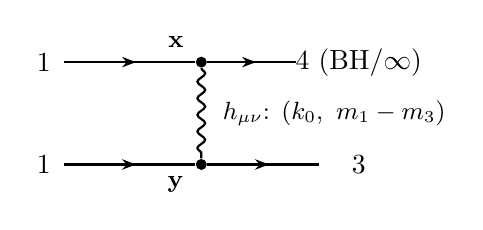
\begin{tikzpicture}
\node[vtx] (x) at (2,1.3) {}; \node[vtx] (y) at (2,0) {};
\node at (0,1.3) {$1$}; \node at (4,1.3) {$4\ ({\rm BH}/\infty)$}; \node at (0,0) {$1$}; \node at (4,0) {$3$};
\draw[psi] (0.25,1.3) -- (x); \draw[psi] (x) -- (3.2,1.3); \draw[psi] (0.25,0) -- (y); \draw[psi] (y) -- (3.5,0);
\draw[grav] (x) -- (y);
\node[right,font=\small] at (2.15,0.65) {$h_{\mu\nu}$: $(k_0,\ m_1-m_3)$};
\node[left,font=\small] at (1.9,1.55) {$\bx$}; \node[left,font=\small] at (1.9,-0.25) {$\by$};
\end{tikzpicture}
\end{center}
Insert $\psi=\sum c_N\psi_N$ into $H_{\rm int}=-L_{\rm eff}$ and keep the terms $\propto\bar c_4\bar c_3c_1c_1$. They come from putting the bilinear $(41)$ at one end of the graviton and $(31)$ at the other, in both orders. Every term below has the same overall combinatorial factor as the Newtonian and SI vertices, so that factor cancels in all ratios:
\begin{align}
A_{\rm N}&=-G\mu^2\!\int\!\!\int\frac{\rho^{41}(\bx)\,\rho^{31}(\by)}{|\bx-\by|}, \label{eq:AN}\\
A_{h_{0i}}&=+4G\!\int\!\!\int\frac{\bj^{41}(\bx)\cdot\bj^{31}(\by)}{|\bx-\by|},\label{eq:AGM}\\
A_{h_{ij}}&=A_{h_{00}[T_{kk}]}=-\frac G2\!\int\!\!\int\frac{\rho^{41}t^{31\prime}+t^{41}\rho^{31\prime}}{|\bx-\by|},\label{eq:Ahij}\\
A_{T_{00}}&=-\frac G2\!\int\!\!\int\frac{\rho^{41}(\nabla\bar\psi_3\!\cdot\!\nabla\psi_1)'+(\nabla\bar\psi_4\!\cdot\!\nabla\psi_1)\rho^{31\prime}}{|\bx-\by|},\\
A_{\rm ret}&=+\frac{G\mu^2k_0^2}{2}\!\int\!\!\int\rho^{41}\rho^{31\prime}\,|\bx-\by|,\qquad k_0=\omega_1-\omega_3,\\
A_{G^2}&=+G^2M\mu^2\!\int\!\!\int\rho^{41}\rho^{31\prime}\Big[\frac1{r_xr_y}+\Big(\frac1{r_x}+\frac1{r_y}\Big)\frac1{|\bx-\by|}\Big].
\end{align}
\begin{verify}[Signs and factors in three lines]
\begin{itemize}[nosep]
\item \textbf{Newton:} $-L\supset-\tfrac G2\int\!\!\int\mu^2|\psi|^2|\psi'|^2/r$, and the two orderings give the factor 2, hence $-G\mu^2$. This reproduces $K_{\rm N}$.
\item \textbf{Gravitomagnetism:} $-L\supset+2G\int\!\!\int T_{0i}T'_{0i}/r=2G\int\!\!\int\bj\cdot\bj'/r$, and the two orderings give $+4G$.
\item \textbf{Retardation:} $1/r\to-\tfrac12k_0^2r$ inside $A_{\rm N}$. The energy through the graviton is the same, $\pm k_0$, in both orderings, because $2\omega_1=\omega_3+\omega_4$.
\end{itemize}
\end{verify}
We report every correction as $\delta_X\equiv A_X/A_{\rm N}$, so $\Gamma_{\rm SG}\to\Gamma_{\rm SG}\,|1+\sum_X\delta_X|^2$.

\subsection{Why we must integrate by parts}
Mode 4 is not a normalisable bound state. It is defined through a Green's function: the existing code (\texttt{gf\_radial}) solves the Klein--Gordon equation on Kerr with a \emph{source} $S(\bx)$ and BH-ingoing or outgoing boundary conditions, and reads off the flux. So we need each amplitude in the form
\[
A_X=\int\dd^3x\;\bar\psi_4(\bx)\,S_X(\bx),
\]
with no derivatives acting on $\psi_4$. Wherever $\nabla\bar\psi_4$ appears, we move the derivative onto the rest by parts. Here are the two worked cases.

\paragraph{Gravitomagnetic term.} Define the gravitomagnetic vector potential of the transition current, $\bA(\bx)=\int\bj^{31}(\by)/|\bx-\by|$, so $A_{h_{0i}}=4G\int\bj^{41}\cdot\bA$. With $\bj^{41}=-\tfrac i2(\bar\psi_4\nabla\psi_1-\psi_1\nabla\bar\psi_4)$ and $\int\psi_1\bA\cdot\nabla\bar\psi_4=-\int\bar\psi_4\nabla\cdot(\psi_1\bA)$:
\[
\int\bj^{41}\cdot\bA=-\tfrac i2\int\bar\psi_4\big[2\bA\cdot\nabla\psi_1+\psi_1\nabla\!\cdot\!\bA\big].
\]
The divergence is fixed by \textbf{particle-number conservation}. The transition current obeys $\partial_t(\mu\rho^{31})+\nabla\cdot\bj^{31}=0$, and $\rho^{31}\propto e^{-ik_0t}$, so $\nabla\cdot\bj^{31}=i\mu k_0\rho^{31}$ and hence $\nabla\cdot\bA=i\mu k_0\Phi$ with $\Phi\equiv\int\rho^{31}/|\bx-\by|$. Altogether
\begin{equation}
S_{h_{0i}}=-4iG\,\bA\cdot\nabla\psi_1+2G\mu k_0\,\psi_1\Phi.
\end{equation}

\paragraph{Stress term, and where a contact term comes from.} Two identities do all the work. The first is $\int f\,\nabla\bar\psi_4\cdot\nabla\psi_1=-\int\bar\psi_4\nabla\cdot(f\nabla\psi_1)$. The second is the Poisson equation in the form $\int\nabla^2\rho(\by)/|\bx-\by|=-4\pi\rho(\bx)$. The $\nabla^2(\bar\psi\psi)$ piece of $t^{BA}$ is a total derivative, but integrated against $1/|\bx-\by|$ it becomes a \emph{local} term. Doing both halves of \eqref{eq:Ahij}:
\begin{equation}
2S_{h_{ij}}=G\Big[-\psi_1\!\int\!\frac{\nabla\bar\psi_3\!\cdot\!\nabla\psi_1}{|\bx-\by|}+\nabla\Phi\cdot\nabla\psi_1+\Phi\,\nabla^2\psi_1\;-\;6\pi\,\psi_1^2\bar\psi_3\Big].
\end{equation}
\begin{idea}[A curiosity]
The last term has exactly the form of the axion's contact interaction, $\psi_1^2\bar\psi_3$. For $h_{ij}$ alone (half of the above) it corresponds to $1/(8f^2)\leftrightarrow3\pi G$. At 1PN, gravity itself generates a small local quartic coupling of the field.
\end{idea}
Newton is simply $S_{\rm N}=-G\mu^2\psi_1\Phi$. The $T_{00}$, retardation and $G^2$ sources follow in the same way (code: \texttt{all\_sources} in \texttt{sg\_1pn.jl}).

\subsection{How the numbers are produced}
\begin{enumerate}[leftmargin=1.4em]
\item \textbf{Potentials by multipoles.} Every potential is a Coulomb-type integral. Expand $1/|\bx-\by|=\sum_{LM}\frac{4\pi}{2L+1}Y_{LM}(\hat\bx)\bar Y_{LM}(\hat\by)\,r_<^L/r_>^{L+1}$, project the density onto $Y_{LM}$ on an $(r,\theta)$ grid (Gauss--Legendre in $\cos\theta$), and do two cumulative radial integrals per $L$. The retardation kernel uses
\[
|\bx-\by|=\sum_LP_L(\cos\gamma)\Big[\frac{r_<^{L+2}}{(2L+3)r_>^{L+1}}-\frac{r_<^{L}}{(2L-1)r_>^{L-1}}\Big].
\]
\item \textbf{Vectors as scalars.} $\bA$ is built from the Cartesian spherical components $j_\pm=j_x\pm ij_y$ and $j_z$. Each has a definite azimuthal number ($m\pm1$ and $m$), so each is a scalar Coulomb problem.
\item \textbf{Projection.} Each source is projected onto mode 4's harmonic, $\int S\,\bar Y_{\ell_4m_4}(r^2+a^2\cos^2\theta)\dd\Omega$. This is the same Kerr ``$\Sigma$'' weighting \texttt{gf\_radial} uses. The resulting radial source is then fed to the unchanged Kerr Green's function.
\item \textbf{Which eigenfunctions.} The corrections are themselves $O(\alpha^2)$, so they are evaluated with hydrogenic eigenfunctions; the error is $O(\alpha^4)$. The Newtonian amplitude they are normalised to uses the same eigenfunctions.
\end{enumerate}
\begin{verify}[How we know the bookkeeping is right]
Replace mode 4 by a \emph{bound} state ($|320\rangle$). Then the original double integrals \eqref{eq:AGM}--\eqref{eq:Ahij}, with derivatives acting on $\psi_4$, can be computed directly. They agree with $\int\bar\psi_4S_X$ to $6\times10^{-7}$ ($h_{0i}$) and $5\times10^{-6}$ (stress). This tests every integration by parts and the continuity step (\texttt{julia sg\_1pn.jl test}).
\end{verify}

%=====================================================================
\section{Lecture 5 --- Estimates first, then numbers}
%=====================================================================

\subsection{Back of the envelope}
Use the point-particle formulas with $v_1\sim\alpha/n_1$ and $v_3\sim\alpha/n_3$ as the speeds ``at the two vertices'':
\begin{itemize}[leftmargin=1.4em]
\item \textbf{$h_{0i}$:} $\delta\sim-4\,\bv_1\!\cdot\bv_3$. Both transition currents inherit the azimuthal flow of the superradiant state 1, so they are \emph{aligned}. Co-moving mass currents \emph{repel} gravitomagnetically (the $-4\bv_1\!\cdot\bv_2$ in EIH), so this term weakens the attraction. Estimate: $-4(\alpha/2)(\alpha/3)=-0.67\alpha^2$ for $211\to322$, and $-4(\alpha/3)(\alpha/5)=-0.27\alpha^2$ for $322/544$.
\item \textbf{$h_{ij}$:} $\delta\sim+\tfrac12(v_1^2+v_3^2)$. Stress adds to the active mass, so this term strengthens the attraction. Estimate: $+0.18\alpha^2$ for $211\to322$, and $+0.08\alpha^2$ for $322/544$.
\item \textbf{Retardation:} $\delta\sim\tfrac12k_0^2r^2$, with $k_0$ a level spacing $\sim\alpha^3/n^3$ in $GM$ units and $r\sim n^2/\alpha^2$. This is small.
\item \textbf{$G^2$:} $\delta\sim-2GM/r\sim-2\alpha^2/n^2$, negative, of the same order as $h_{0i}$.
\end{itemize}

\subsection{The numbers}
\begin{figure}[h]
\centering
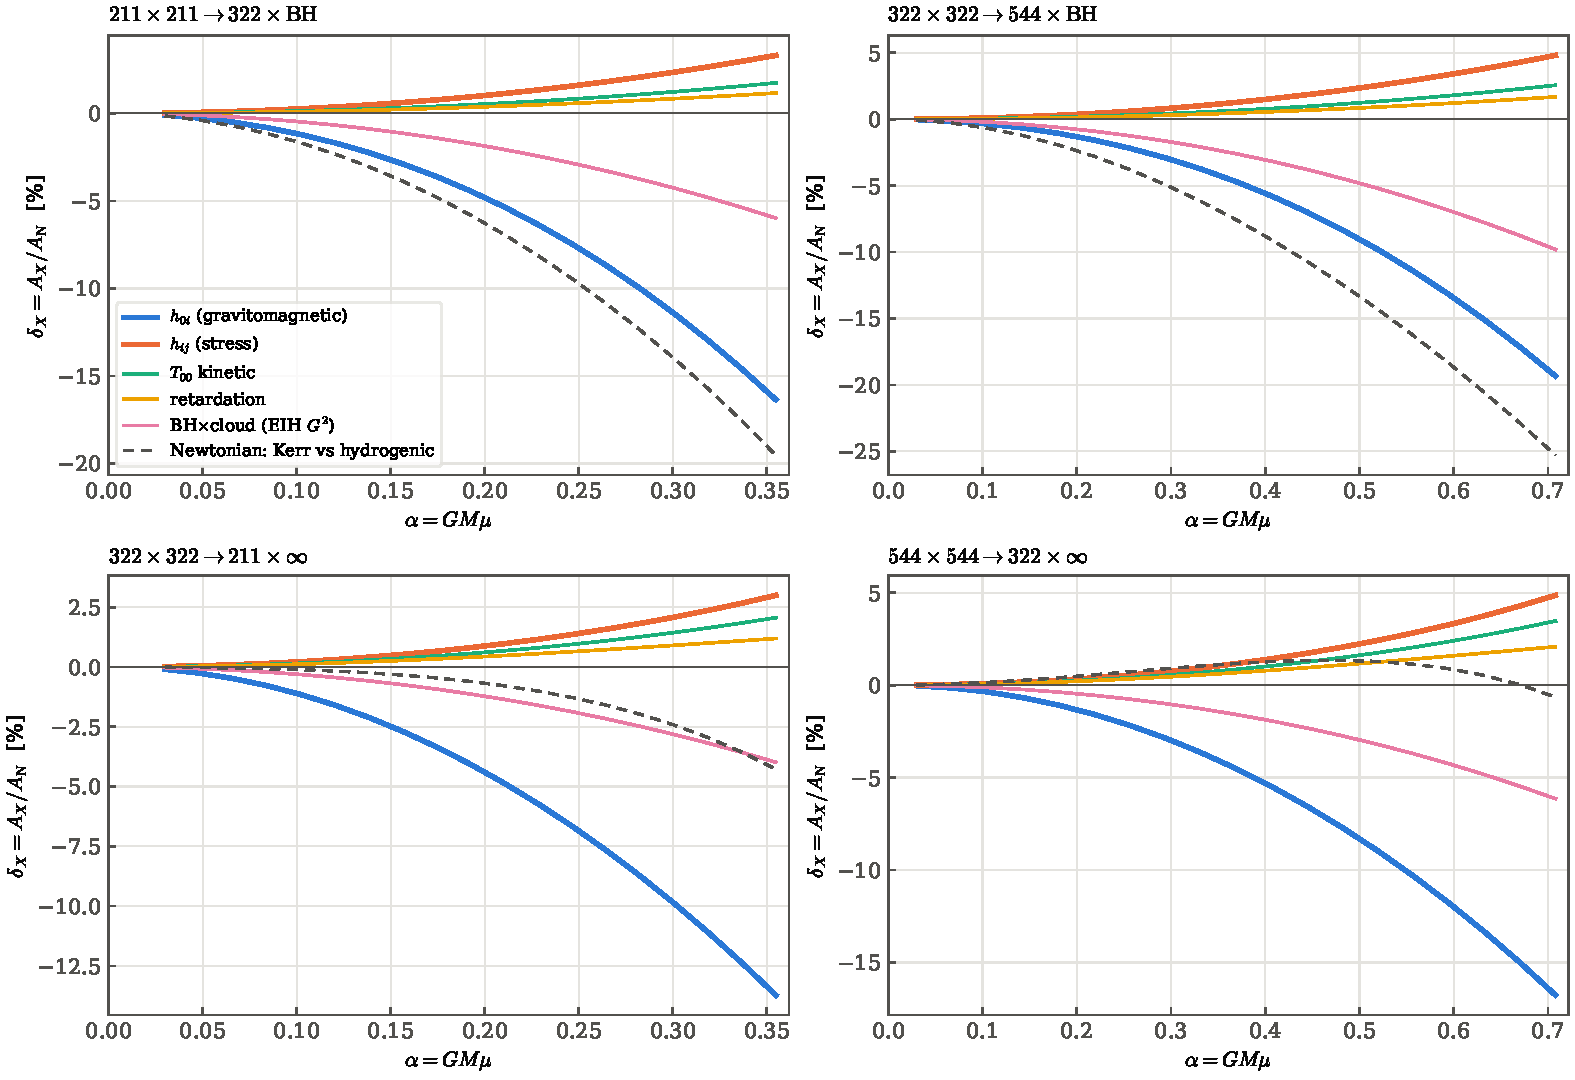
\includegraphics[width=\textwidth]{fig_1pn.pdf}
\caption{Fractional corrections $\delta_X=A_X/A_{\rm N}$ to the Newtonian self-gravity amplitude (Kerr Green's function, $\tilde a=0.95$). Thick lines: $h_{0i}$ and $h_{ij}$. The $h_{ij}$ line is $h_{ij}$ alone; the stress-sourced $h_{00}$ adds an identical amount. Dashed: change of the \emph{Newtonian} amplitude when Kerr instead of hydrogenic eigenfunctions are used, $\sqrt{C_{\rm Kerr}/C_{\rm hyd}}-1$, a stand-in for the $O(\alpha^2)$ effects on the wavefunction side.}
\label{fig:1pn}
\end{figure}

\begin{table}[h]
\centering\small
\begin{tabular}{@{}lcccccc@{}}
\toprule
channel & $h_{0i}$ & $h_{ij}$ & $T_{00}$ & ret. & $G^2$ BH$\times$cloud & sum$^\dagger$\\\midrule
$211\times211\to322\times{\rm BH}$ & $-1.14$ & $+0.25$ & $+0.13$ & $+0.10$ & $-0.46$ & $-0.87$ \\
$322\times322\to544\times{\rm BH}$ & $-0.32$ & $+0.09$ & $+0.05$ & $+0.03$ & $-0.19$ & $-0.24$ \\
$322\times322\to211\times\infty$ & $-1.10$ & $+0.21$ & $+0.15$ & $+0.12$ & $-0.30$ & $-0.72$ \\
$544\times544\to322\times\infty$ & $-0.33$ & $+0.08$ & $+0.06$ & $+0.05$ & $-0.11$ & $-0.17$ \\

\bottomrule
\end{tabular}
\caption{Small-$\alpha$ coefficients $\delta_X/\alpha^2$ at $\alpha=0.03$. Compare with the estimates: $h_{0i}$: $-1.1$ vs $-0.67$ and $-0.32$ vs $-0.27$; $h_{ij}$: $+0.25$ vs $+0.18$ and $+0.09$ vs $+0.08$. $^\dagger$Sum $=h_{0i}+2h_{ij}+T_{00}+{\rm ret}+G^2$.}
\label{tab:coeffs}
\end{table}

\begin{table}[h]
\centering\small
\begin{tabular}{@{}lcccccc@{}}
\toprule
channel & $\alpha$ & $\delta_{h_{0i}}$ [\%] & $\delta_{h_{ij}}$ [\%] & $\Delta\Gamma_{\rm SG}$ ($h_{0i}$) [\%] & ($h_{ij}$) [\%] & sum$^\dagger$ [\%]\\\midrule
$211\times211\to322\times{\rm BH}$ & $0.30$ & $-11.4$ & $+2.4$ & $-22$ & $+5$ & $-8.9$ \\
$322\times322\to544\times{\rm BH}$ & $0.29$ & $-2.9$ & $+0.8$ & $-6$ & $+2$ & $-2.2$ \\
$322\times322\to211\times\infty$ & $0.30$ & $-9.9$ & $+2.1$ & $-19$ & $+4$ & $-6.2$ \\
$544\times544\to322\times\infty$ & $0.29$ & $-2.9$ & $+0.7$ & $-6$ & $+1$ & $-1.4$ \\

\bottomrule
\end{tabular}
\caption{Values at $\alpha\simeq0.3$; $\Delta\Gamma_{\rm SG}=|1+\delta|^2-1$.}
\label{tab:values}
\end{table}

\subsection{What we learned}
\begin{enumerate}[leftmargin=1.4em]
\item \textbf{$h_{0i}$ is the biggest 1PN effect}, and it is negative. It reduces $\Gamma_{\rm SG}$ by $\simeq20\%$ at $\alpha=0.3$ for $211\times211\to322\times{\rm BH}$ and $322\times322\to211\times\infty$, and by $\simeq6\%$ for the $322/544$ channels. The higher-$n$ states move more slowly, hence the smaller effect.
\item \textbf{$h_{ij}$ is $\sim5\times$ smaller and positive}, as estimated.
\item \textbf{The $G^2$ terms are the second largest} and negative. Retardation and $T_{00}$ are at the percent level.
\item \textbf{Consequence for SG vs SI.} $\Gamma_{\rm SG}/\Gamma_{\rm SI}\propto C$ and the crossover $f_a\propto C^{-1/4}$. The summed correction ($-9\%$ in amplitude at $\alpha=0.3$ for the $211$ channel) therefore moves the crossover by only $\lesssim5\%$, and by $\lesssim10\%$ over each channel's full $\alpha$ range.
\item \textbf{Accuracy.} The graviton-side corrections are comparable to the wavefunction-side ones (dashed line). Quoting $\Gamma_{\rm SG}$ to better than $\sim20\%$ at $\alpha\gtrsim0.3$ needs a consistent treatment of both, which leads to the last lecture.
\end{enumerate}

%=====================================================================
\section{Lecture 6 --- Can we avoid the post-Newtonian expansion altogether?}
%=====================================================================

\textbf{Yes.} The PN expansion was only a device to evaluate one object: \emph{the exchange of a single graviton between two transition stress tensors}, in the background spacetime of the black hole. Linear order in $h$ is exact to first order in the cloud mass $q_c$, which is all we need. What we approximated was the graviton's propagation (flat space plus $G^2$ corrections) and the stress tensors (expanded in $v$). Both can be done exactly.

\subsection{The exact statement}
\begin{enumerate}[leftmargin=1.4em]
\item Build the \textbf{full transition stress tensor} from the Kerr eigenmodes, with no NR expansion:
\[
T^{31}_{\mu\nu}=\partial_{(\mu}\bar\phi_3\,\partial_{\nu)}\phi_1-g_{\mu\nu}\big[\tfrac12g^{\alpha\beta}\partial_\alpha\bar\phi_3\partial_\beta\phi_1+\tfrac12\mu^2\bar\phi_3\phi_1\big],
\]
which oscillates at $k_0=\omega_1-\omega_3$ with azimuthal number $m_1-m_3$.
\item \textbf{Solve the linearised Einstein equations on Kerr}, $\delta G_{\mu\nu}[h]=8\pi G\,T^{31}_{\mu\nu}$, at that single frequency and azimuthal number, with physical boundary conditions (ingoing at the horizon, outgoing at infinity).
\item \textbf{Couple to the other vertex.} The perturbed metric changes the Klein--Gordon operator. The source for mode 4 is
\[
S_4=-\,\delta\Box[h]\,\phi_1,\qquad\delta\Box[h]\,\phi=-h^{\mu\nu}\nabla_\mu\nabla_\nu\phi-\big(\nabla_\mu h^{\mu\nu}-\tfrac12\nabla^\nu h\big)\nabla_\nu\phi,
\]
and it is fed to the \emph{same} Kerr Green's function as now.
\end{enumerate}
This contains Newton, all PN orders, the $G^2$ terms (graviton propagation on the curved background) and frame dragging. Being an on-shell amplitude, it is \textbf{gauge invariant}, which resolves the ambiguity of the individual PN pieces.

\subsection{How to solve step 2 in practice}
This is a standard problem of black-hole perturbation theory, the same machinery used for extreme-mass-ratio inspirals and gravitational self-force. Our source is an extended, smooth cloud rather than a point particle, which actually makes it \emph{easier}.
\begin{itemize}[leftmargin=1.4em]
\item \textbf{Schwarzschild first ($a=0$).} Decompose $h$ and $T$ in tensor harmonics. The odd and even sectors reduce to the Regge--Wheeler and Zerilli master equations with sources, from which $h$ is reconstructed. Alternatively, solve directly in Lorenz gauge, frequency domain (Barack--Lousto; Akcay). The low multipoles $\ell=0,1$ need separate treatment, and they matter: the $211$--$322$ transition density is largely dipolar.
\item \textbf{Kerr.} Solve the Teukolsky equation for $\psi_0$ or $\psi_4$ (spin $\pm2$) with the source built from $T^{31}_{\mu\nu}$. Then reconstruct $h$ in a radiation gauge (Chrzanowski--Cohen--Kegeles), including the corrector needed inside an extended source (Green--Hollands--Zimmerman) and the mass and angular-momentum completion. Alternatively, use the recently developed separable Lorenz-gauge construction on Kerr (Dolan, Kavanagh, Wardell et al.).
\item \textbf{Tools.} Black Hole Perturbation Toolkit. \texttt{GeneralizedSasakiNakamura.jl}, for spin $\pm2$ Teukolsky radial functions in Julia, is by the author of \texttt{SpinWeightedSpheroidalHarmonics.jl}, which the code already uses. The existing \texttt{gw\_rates.jl} already solves the \emph{radiative} part of this problem (the flux of $\psi_4$ to infinity). What is new is the metric \emph{inside} the source region.
\end{itemize}

\subsection{Why it is tractable for us}
\begin{itemize}[leftmargin=1.4em]
\item \textbf{Quasi-static.} The graviton frequency is a level spacing, $k_0\ll1/r_{\rm cloud}$, so we are deep in the near zone and the frequency-domain equations are nearly elliptic.
\item \textbf{Far from the hole.} The cloud lives at $r\sim n^2GM/\alpha^2\gg GM$, so the multipole sums converge fast and the horizon boundary condition matters little.
\item \textbf{Spin is a small effect.} The Newtonian rate changes by $<1\%$ between $\tilde a=0.5$ and $0.95$, and spin-dependent gravity starts at 1.5PN. A Schwarzschild calculation of the graviton propagation, combined with the Kerr eigenfunctions and Green's function already in the code, captures almost everything.
\end{itemize}

\subsection{How we would know it is right}
\begin{itemize}[leftmargin=1.4em]
\item At small $\alpha$ it must reduce to Newton plus the sum of the 1PN pieces computed here, once the eigenfunctions are expressed in the same (harmonic) coordinates.
\item Doing step 2 in two gauges (Regge--Wheeler and Lorenz) must give the same amplitude.
\end{itemize}

\subsection{Other routes, and why we would not take them}
\begin{itemize}[leftmargin=1.4em]
\item \textbf{Flat-space graviton with relativistic stress tensors.} This drops the $G^2$ terms, which are the same order as everything else, so it is not a consistent improvement.
\item \textbf{Full numerical relativity of Einstein--Klein--Gordon.} This is used for self-gravitating cloud spectra (e.g.\ May et al.\ 2024, which Bo\v{s}kovi\'c--Savi\'c compare to). It is exact even beyond linear order in $q_c$, but extracting $2\to2$ rates over a grid of $\alpha$ is impractically expensive, and linear order in $q_c$ is all we need.
\end{itemize}

\begin{result}[Bottom line]
The PN corrections computed here show the size of the effect: $\sim20\%$ in $\Gamma_{\rm SG}$ at $\alpha=0.3$ for the $211$ channel, and less for higher $n$. They are too small to change the SG-vs-SI picture. If percent-level $\Gamma_{\rm SG}$ is ever needed at large $\alpha$, the clean route is the exact one-graviton exchange on Kerr: Schwarzschild propagation first, reusing the existing Kerr eigenfunctions and Green's function.
\end{result}

\appendix
\section{Sign and index dictionary}
\begin{itemize}[nosep,leftmargin=1.4em]
\item $\eta={\rm diag}(-1,1,1,1)$; $T^{00}=T_{00}$, $T^{0i}=-T_{0i}$, $T^{ij}=T_{ij}$; $T=-T_{00}+T_{kk}$.
\item Dust: $T^{00}=\rho$, $T^{0i}=\rho v^i$, so $T_{0i}=-\rho v^i$; $T^{ij}=\rho v^iv^j$.
\item $\Phi=-G\int\rho/r$: $h_{00}=-2\Phi$, $h_{ij}=-2\Phi\delta_{ij}$, $g_{00}=-(1+2\Phi)$.
\item $\nabla^2(1/r)=-4\pi\delta^3$; $\nabla^2r=2/r$.
\item $L=-V$: a positive term in $L_{\rm eff}$ is attractive.
\end{itemize}

\section{Code map}
\begin{itemize}[nosep,leftmargin=1.4em]
\item \texttt{sg\_1pn.jl}:
\begin{itemize}[nosep]
\item \texttt{hyd\_state}: hydrogenic $\psi$, $\nabla\psi$, $\nabla^2\psi$ on the grid.
\item \texttt{coulomb} and \texttt{linear\_kernel}: the $1/r$ and $r$ kernels.
\item \texttt{cart}: spherical $\to$ Cartesian-spherical components.
\item \texttt{all\_sources}: $S_X$ for every piece.
\item \texttt{point\_1pn}: projection and Green's function.
\item \texttt{selftest}.
\end{itemize}
\item \texttt{sg\_vs\_si.jl}: \texttt{gf\_amplitudes}, the Kerr Green's function copied from \texttt{gf\_radial}.
\item \texttt{plot\_1pn.py}: figure and tables of this note.
\end{itemize}

\section{Code fixes made alongside these notes}
\sloppy
\begin{itemize}[leftmargin=1.4em]
\item \texttt{spheroidals} now takes \texttt{alph} and uses the massive-field spheroidicity $c=a\sqrt{\omega^2-\mu^2}$. It previously used $c=a\omega$, the massless convention of \texttt{SpinWeightedSpheroidalHarmonics}. Call sites that had passed $\omega$ in eV now pass dimensionless energies. Effect on \texttt{gf\_radial}: $+0.08\%$ to $+2.1\%$.
\item The $\infty$-channel flux radius in \texttt{gf\_radial} is now $r(r_*)$, not $r(r(r_*))$ (with the above, $+0.7\%$ for $322\times322\to211\times\infty$ at $\alpha=0.17$).
\end{itemize}
Commit \texttt{a9bba4b} on \texttt{gw-signatures}.

\end{document}
